\documentclass{agujournal2019-navid}

\graphicspath{ {figures/} }
\usepackage{lineno,layouts,microtype}


% \linenumbers

\newcommand{\navidcomment}[1]{{\color{red} [#1]}}
\newcommand{\andycomment}[1]{{\color{Green} [#1]}}

%\usepackage[T1]{fontenc}
\renewcommand*\familydefault{\sfdefault} 
\usepackage{sansmath} 
\sansmath

\newcommand{\mathbfit}[1]{\textbf{\textit{\textsf{#1}}}}
\usepackage{amsfonts, amssymb, amsmath}
\usepackage[labelfont=bf]{caption}
% \usepackage{doi}

\usepackage{comment}

%%%%%%%
% As of 2018 we recommend use of the TrackChanges package to mark revisions.
% The trackchanges package adds five new LaTeX commands:
%
%  \note[editor]{The note}
%  \annote[editor]{Text to annotate}{The note}
%  \add[editor]{Text to add}
%  \remove[editor]{Text to remove}
%  \change[editor]{Text to remove}{Text to add}
%
% complete documentation is here: http://trackchanges.sourceforge.net/
%%%%%%%


%% Enter journal name below.
%% Choose from this list of Journals:
%
% JGR: Atmospheres
% JGR: Biogeosciences
% JGR: Earth Surface
% JGR: Oceans
% JGR: Planets
% JGR: Solid Earth
% JGR: Space Physics
% Global Biogeochemical Cycles
% Geophysical Research Letters
% Paleoceanography and Paleoclimatology
% Radio Science
% Reviews of Geophysics
% Tectonics
% Space Weather
% Water Resources Research
% Geochemistry, Geophysics, Geosystems
% Journal of Advances in Modeling Earth Systems (JAMES)
% Earth's Future
% Earth and Space Science
% Geohealth
%
% ie, \journalname{Water Resources Research}

% \journalname{Geophysical Research Letters}

\usepackage{scalerel, stackengine}
\setstackEOL{\#}
\stackMath
\def\hatgap{2pt}
\def\subdown{-2pt}
\newcommand\reallywidehat[2][]{ \renewcommand\stackalignment{l} \stackon[\hatgap]{#2}{ \stretchto{
    \scalerel*[\widthof{$#2$}]{\kern-.6pt\bigwedge\kern-.6pt}
    {\rule[-\textheight/2]{1ex}{\textheight}}}
    {0.5ex}_{\smash{ \belowbaseline[\subdown]{\scriptstyle#1} }}
}}


%% MACROS

% Vector calculus 
  \newcommand{\p}		{\partial}
  \newcommand{\bnabla}	{\boldsymbol \nabla}
  \newcommand{\grad}	{\bnabla}
\renewcommand{\div}	    {\bnabla \bcdot}
  \newcommand{\bcdot}	{\boldsymbol \cdot}
  \newcommand{\lap}		{\triangle}

% Boldsymbols
\newcommand{\bu}		{\boldsymbol{u}}
\newcommand{\bx}		{\mathbfit x}
\newcommand{\bU}		{\mathbfit{U}}
\newcommand{\bX}		{\mathbfit{X}}
\newcommand{\bxh}		{\hspace{0.1em} \boldsymbol{\hat x}}
\newcommand{\byh}		{\hspace{0.1em}\boldsymbol{\hat y}}
\newcommand{\bzh}		{\hspace{0.1em}\boldsymbol{\hat z}}
\newcommand{\bnh}		{\hspace{0.1em}\boldsymbol{\hat n}}
\newcommand{\bxi}		{\ensuremath {\boldsymbol {\xi}}}

% Greek
\newcommand{\ep}		{\epsilon}
\newcommand{\om}		{\omega}
\newcommand{\kap}		{\kappa}
\newcommand{\sig}		{\sigma}
\newcommand{\gam}	  {\gamma}
\newcommand{\lam}		{\lambda}

% Romans
\newcommand{\ee}		{\mathrm{e}}
\newcommand{\ii}		{\mathrm{i}}
\newcommand{\dd}		{{\rm d}}
\newcommand{\id}		{{\, \rm d}}

% Misc
\newcommand{\Dt}[1]	    {\mathrm{D}_t #1}
\newcommand{\half}		{\tfrac{1}{2}}
\newcommand{\where}	    {\qquad \text{where} \qquad}
\newcommand{\andand}	{\qquad \text{and} \qquad}
\newcommand{\com}		{\, ,}
\newcommand{\per}		{\, .}
\newcommand{\defn}	    {\ensuremath{\stackrel{\mathrm{def}}{=}}}
\renewcommand{\equiv} {\ensuremath{\stackrel{\mathrm{def}}{=}}}
\newcommand{\av}[1]	    {\left \langle {#1} \right \rangle}
\newcommand{\beq}		{\begin{equation}}
\newcommand{\eeq}		{\end{equation}}
\newcommand{\Pa}		{\mathrm{N}\,\mathrm{m}^{-2}}
\newcommand{\rhom} {\rho_{\mathrm{m}}}
\newcommand{\ws} {\mathrm{WS}}
\newcommand{\tfs} {\mathrm{TFS}}
\newcommand{\ifs} {\mathrm{IFS}}
\newcommand{\bd} {\mathrm{BD}}
\newcommand{\hb} {h_{\mathrm{bot}}}
\newcommand{\pb} {p_{\mathrm{bot}}}



\hypersetup{
	breaklinks,
	colorlinks=true,
	linkcolor=Blue,
  urlcolor=Purple,
	citecolor=Purple,
%	allcolors=black,
	pdfauthor={N. C. Constantinou and A. McC. Hogg}
 }


\begin{document}
\justify
\title{Circumpolar variations in Southern Ocean eddy dynamics:\\An ensemble approach}

\authors{
Andrew McC. Hogg\affil{1}, Thierry Penduff\affil{2}, Sally E. Close\affil{3}, William K. Dewar\affil{4},\\Navid C. Constantinou\affil{1}\quad and\quad Josu{\'e} Mart{\'i}nez Moreno\affil{1}
}

\affiliation{1}{Research School of Earth Sciences and ARC Centre of Excellence for Climate Extremes,\\ Australian National University, Australia}
\affiliation{2}{Universit{\'e} Grenoble Alpes, CNRS, IRD, Grenoble-INP, IGE, Grenoble, France}
\affiliation{3}{Institut des Géosciences de l'Environnement, CNRS/Univ. Grenoble Alpes/G-INP/IRD, France}
\affiliation{3}{Florida State University, Tallahassee, FL, USA}

\correspondingauthor{Andrew McC. Hogg}{Andy.Hogg@anu.edu.au}

\begin{keypoints}
\item Variations in the Southern Ocean eddy field are dominated by intrinsic, rather than forced, processes.
\item The forced component of the the variance is governed by the local wind stress input.
\item The eddy field lags variations in wind stress, with two clear timescales emerging: one at 6-9 months, which we attribute to baroclinic instability, and one at 2-3 years, which we attribute to the delayed effect of topographic steering.
\end{keypoints}

\begin{abstract}
Circulation in the Southern Ocean is unique in global ocean.
The strong wind stress forcing and buoyancy fluxes, in concert with the lack of continental boundaries, conspire to drive the Antarctic Circumpolar Current replete with an intense eddy field.
The effect of Southern Ocean eddies on the ocean circulation is significant -- they modulate the momentum balance of the zonal flow, and the meridional transport of tracers and mass.
The strength of the eddy field is controlled by a combination of forcing (primarily thought to be wind stress) and intrinsic variability associated with the turbulent flow field itself.
Here, we present results from an eddy-permitting ensemble of ocean model simulations to investigate the relative contribution of forcing and intrinsic processes in governing the variability of the Southern Ocean eddy field.
We find that intrinsic processes dominate the eddy field.
Where correlations between the forcing and the eddy field exist, these interactions are dominated by two distinct timescale -- a fast baroclinic instability response; and a multi-year process owing to feedback between bathymetry and the mean flow.
These results suggest that understanding Southern Ocean eddy dynamics requires an ensemble approach to eliminate intrinsic variability, and therefore may not yield robust conclusions from observations alone.

\noindent \textbf{Plain language summary} \\
\noindent The Southern Ocean is the most turbulent region of the world's oceans.
The variations in this turbulence, which is often referred to as \emph{eddies}, is critical to understanding the evolution of the Southern Ocean under climate change.
But it's hard to get information about these eddies, because they occur on small scales in a large ocean basin that is poorly observed.
In addition, the observational record is quite short, which makes it more difficult to use these observations to study what controls variation in the eddy field.
For this reason, we take an eddy-permitting ocean model, and run it 50 times with the same forcing (but a slightly different initial state).
The chaotic nature of the turbulent ocean means that these models runs diverge into different states.
We thus use these simulations to study which eddy processes are intrinsic (that is, a consequence of the chaotic nature of turbulence) and which are forced by the external forcing that is common to all experiments (such as wind forcing).
We conclude that the Southern Ocean eddy field is dominated by intrinsic chaotic processes; but that the forced variability responds to wind on particular timescales that are controlled by the mechanisms that generate ocean turbulence. 
\end{abstract}




%% ------------------------------------------------------------------------ %%
%
%  TEXT
%
%% ------------------------------------------------------------------------ %%

\section{Introduction}

Southern Ocean eddies are important to the climate response - for compensation, saturation, etc.

Proxy for eddy strength is Transient KE (TKE), often called eddy KE. Define.

TKE responds to variations in wind stress forcing, but with a lag. Studied by many. This lag is relevant for eddy saturation and LFV.

Confusion about what this lag might be. It seems to be event- and region-dependent. Also, not clear whether it emerges from the noise in either model simulations or observations.

So, let’s reduce the noise with an ensemble approach. Look at both SO-wide and regional responses.


\section{Methods}

Model description (Thierry)

OCCIPUT strategy (Thierry)

Calculating geouv from SSH, removing trends, etc. (Sally)

Paragraph on TKE and filtering  to eliminate seasonal signal (Andy)

Paragraph on intrinsic-forced ratio and its limitations.


\section{Results}

\begin{figure}[t]
\begin{center}
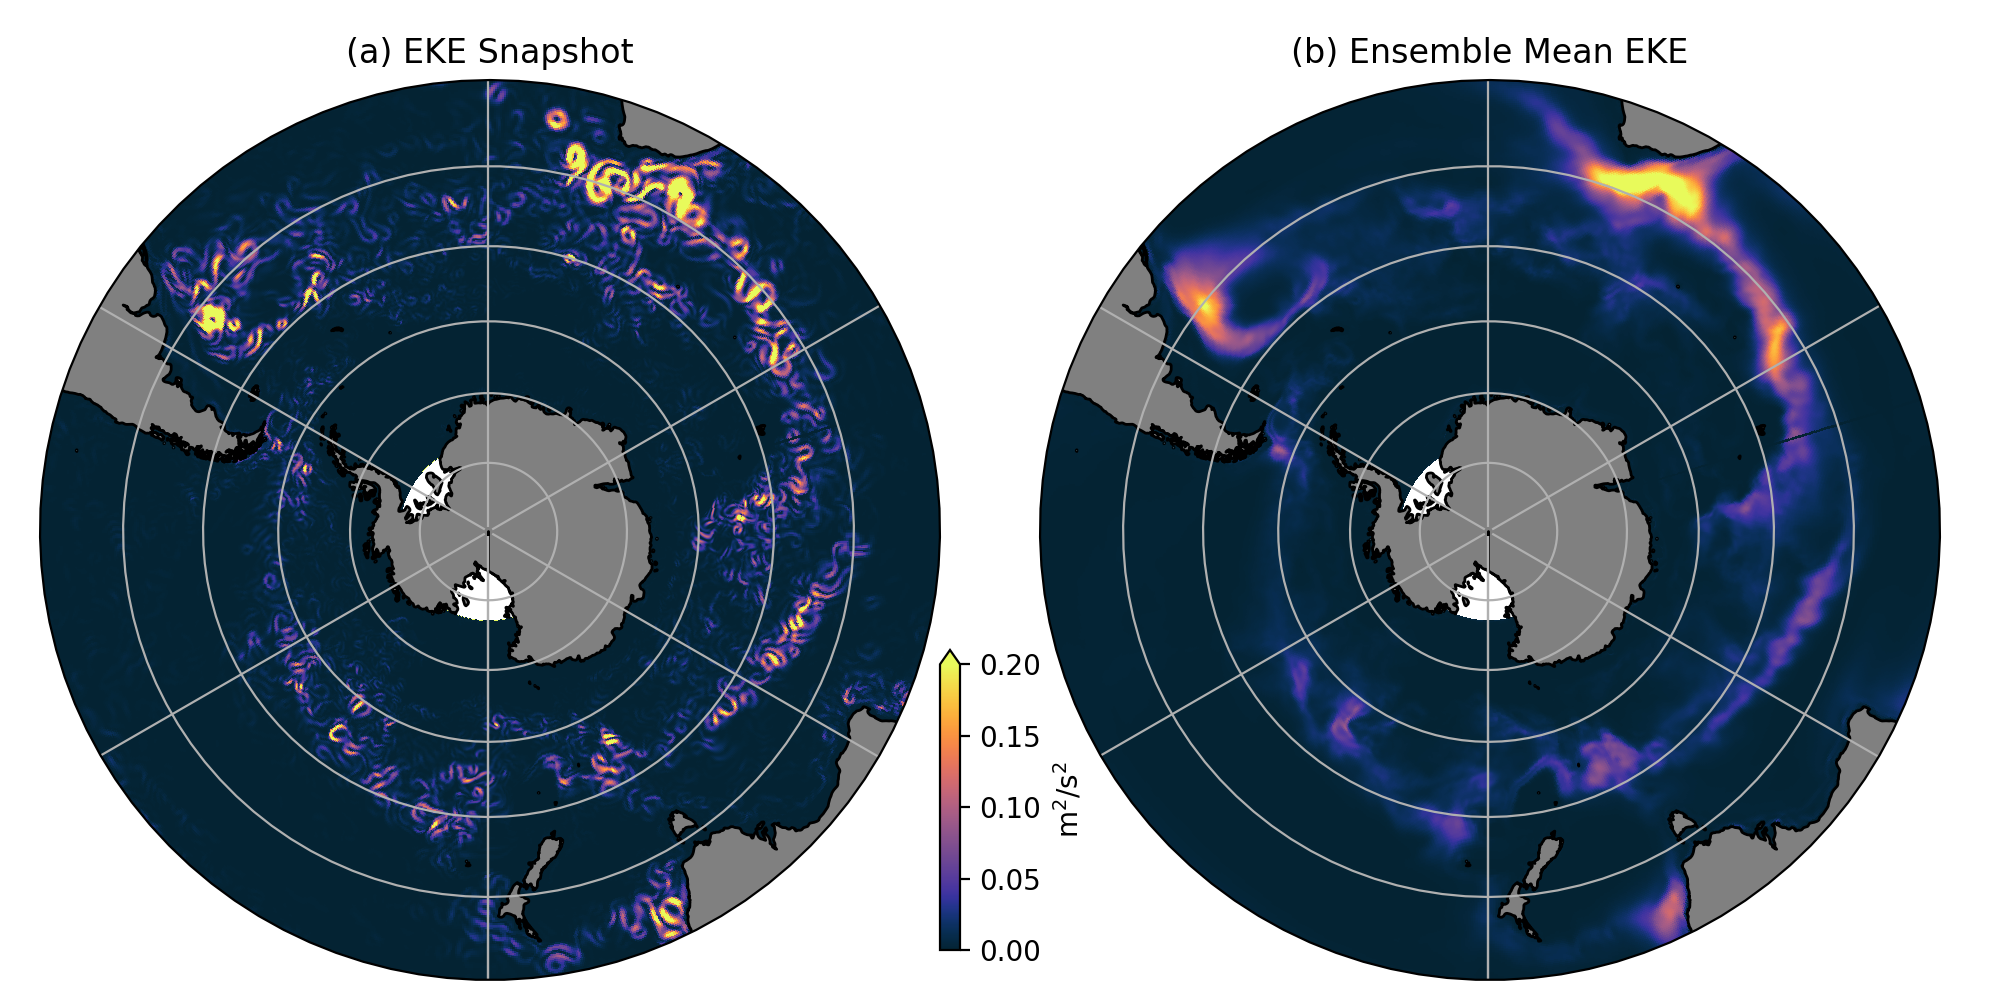
\includegraphics[width=\hsize]{Figure1}
\caption{(a) EKE snapshot and (b) ensemble mean EKE  }
\label{default}
\end{center}
\end{figure}

Figure 2 - Entire Southern Ocean:(a,b) cherrypicked experiments TKE + lag; (c) ensemble mean TKE + lag

Figure 3 - 4 or 6 sectors TKE + lag

Figure 4 - interesting regions - again 4 or 6 of them, TKE + lags

Figure 5 - Ri ratio plot, and other global features

\section{Discussion}
How do we interpret intrinsic variance ratio in this case?

What can we infer about real world?

Propose hypotheses for two timescales (do we need to test these at all?)



\section{Conclusions}
\begin{itemize}
    \item Intrinsic variance is large.
    \item  Forced component exists and has two timescales.
    \item Short timescale is local eddy response - mixed  barotropic/baroclinic?
    \item Long timescale requires topographic feedback.

\end{itemize}



\acknowledgments
We acknowledge NCI for everything they do for us.

\bibliography{basic_references}

\end{document}